\documentclass{article}\usepackage[]{graphicx}\usepackage[]{color}
% maxwidth is the original width if it is less than linewidth
% otherwise use linewidth (to make sure the graphics do not exceed the margin)
\makeatletter
\def\maxwidth{ %
  \ifdim\Gin@nat@width>\linewidth
    \linewidth
  \else
    \Gin@nat@width
  \fi
}
\makeatother

\definecolor{fgcolor}{rgb}{0.345, 0.345, 0.345}
\newcommand{\hlnum}[1]{\textcolor[rgb]{0.686,0.059,0.569}{#1}}%
\newcommand{\hlstr}[1]{\textcolor[rgb]{0.192,0.494,0.8}{#1}}%
\newcommand{\hlcom}[1]{\textcolor[rgb]{0.678,0.584,0.686}{\textit{#1}}}%
\newcommand{\hlopt}[1]{\textcolor[rgb]{0,0,0}{#1}}%
\newcommand{\hlstd}[1]{\textcolor[rgb]{0.345,0.345,0.345}{#1}}%
\newcommand{\hlkwa}[1]{\textcolor[rgb]{0.161,0.373,0.58}{\textbf{#1}}}%
\newcommand{\hlkwb}[1]{\textcolor[rgb]{0.69,0.353,0.396}{#1}}%
\newcommand{\hlkwc}[1]{\textcolor[rgb]{0.333,0.667,0.333}{#1}}%
\newcommand{\hlkwd}[1]{\textcolor[rgb]{0.737,0.353,0.396}{\textbf{#1}}}%
\let\hlipl\hlkwb

\usepackage{framed}
\makeatletter
\newenvironment{kframe}{%
 \def\at@end@of@kframe{}%
 \ifinner\ifhmode%
  \def\at@end@of@kframe{\end{minipage}}%
  \begin{minipage}{\columnwidth}%
 \fi\fi%
 \def\FrameCommand##1{\hskip\@totalleftmargin \hskip-\fboxsep
 \colorbox{shadecolor}{##1}\hskip-\fboxsep
     % There is no \\@totalrightmargin, so:
     \hskip-\linewidth \hskip-\@totalleftmargin \hskip\columnwidth}%
 \MakeFramed {\advance\hsize-\width
   \@totalleftmargin\z@ \linewidth\hsize
   \@setminipage}}%
 {\par\unskip\endMakeFramed%
 \at@end@of@kframe}
\makeatother

\definecolor{shadecolor}{rgb}{.97, .97, .97}
\definecolor{messagecolor}{rgb}{0, 0, 0}
\definecolor{warningcolor}{rgb}{1, 0, 1}
\definecolor{errorcolor}{rgb}{1, 0, 0}
\newenvironment{knitrout}{}{} % an empty environment to be redefined in TeX

\usepackage{alltt}

\usepackage{amsmath,amssymb}
\usepackage[margin =0.51in]{geometry}
\usepackage{enumitem}
\usepackage{parskip}
\usepackage{hyperref}
\IfFileExists{upquote.sty}{\usepackage{upquote}}{}
\begin{document}

\title{Pretrial analysis: thoughts and issues}
\author{mike freund}
\date{\today}
\maketitle


\section*{hypotheses}

\begin{itemize}
  \item During mostly incongruent lists (proactive), subjects are preparing in advance of stimulus onset for the occurrence of an incongruent stimulus
  \item In contrast, during mostly congruent lists (baseline), no preparation occurs.
  \item Neural coding underlying this preparation is to some degree abstract, i.e., generalizes across particular stimuli (e.g., bias items or PC50 items).
  \item Neural coding underlying this preparation involves predictive coding of congruency---i.e., a `pre-activation' of target-evoked congruency representations.
\end{itemize}


\section*{approach}

Approach problem via ``temporal generalization'' method.
See ADD REF.

\begin{itemize}
  \item Train decoders at different TRs peri-stimulus onset to classify incongruent versus congruent patterns.
  \item Test each decoder at each TR.
  \item Use continuous measure of decoding strength / classifier evidence; e.g., distance to bound.
  \item Arrange results in TR by TR confusion matrix.
\end{itemize}



\begin{knitrout}
\definecolor{shadecolor}{rgb}{0.969, 0.969, 0.969}\color{fgcolor}
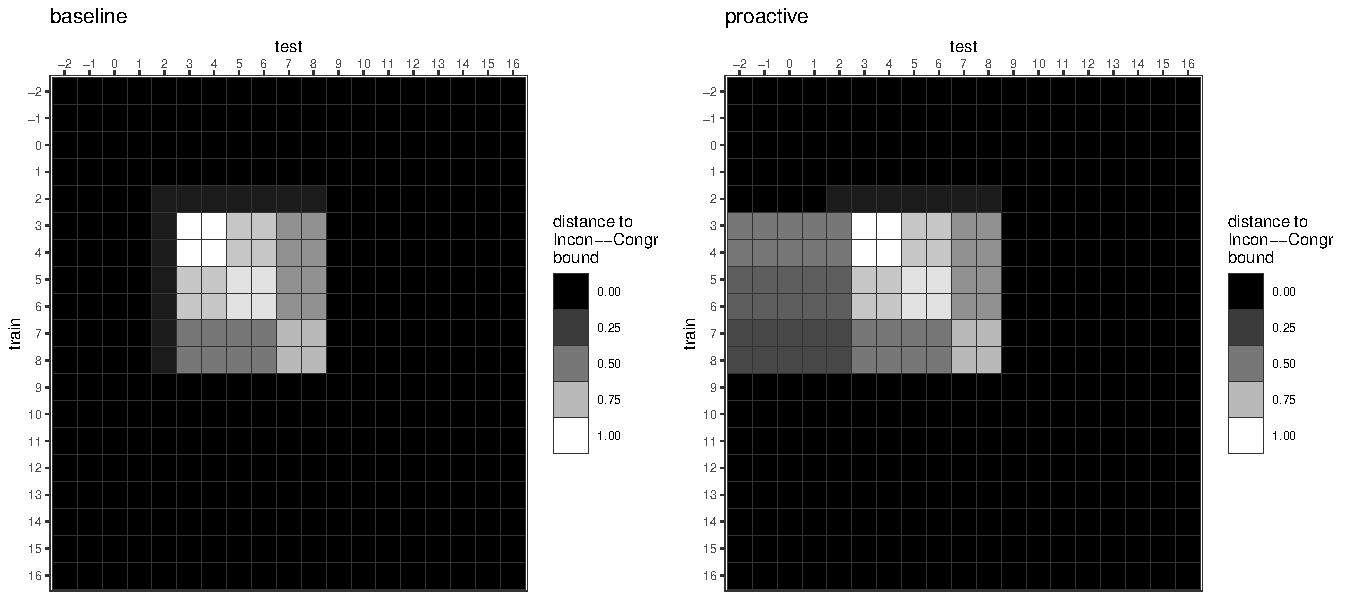
\includegraphics[width=\maxwidth]{figure/unnamed-chunk-1-1} 

\end{knitrout}


\begin{itemize}
  \item Rows indicate the TR / knot at which the decoder was TRAINED; Cols indicate the TR / knot at which the decoder was TESTED.
  \item ``Target knots'' (i.e., peak $\text{high} = \text{low}$ univariate resonse) assumed to be TRs 3 and 4.
\end{itemize}


% pretrial analyses
% ---
% 
% issues
% 	- diffs in template strength btw bas and pro
% 	- method:
% 		model-free (SVM / LDA / Corr)
% 			train: run 1, I--C
% 			test: detrended resids run 2 across trials
% 				- split: prev I prev C
% 		model-based
% 			- pretrial knots estimated
% 				->
% 			- regressors split by prev I and prev C
% 			train: run 1, I--C, all TRs
% 			test: run 2, I--C, all TRs
% 			

\section*{plan}

\begin{itemize}
  \item glm-free versus glm-based method
    
    \begin{itemize}
      \item assess prev*current trial.type counts per session*subj*run
      \item  build xmats with extended event models (1tr1knot); experiment with number of pretrial TRs and duration of events --- colliniarity?
    \end{itemize}
    
  \item if glm-based method viable
  
  \begin{itemize}
    \item fit baseline and event model
    \item generate diagonal.
    linear discriminant function: project 'unlabeled' beta pattern vectors. 
    negate congruent patterns, so positive indicates (correct) distance from bound. 
    validate with correlation decoder; difference between templates.
    should observe clear peak at target TRs. 
    make list of ROIs.
    \item generate off-diagonals.
  \end{itemize}
  
  \item if glm-based method not viable.
  
  \begin{itemize}
    \item ...
    \item 
    \item 
  \end{itemize}
  
\end{itemize}





\end{document}
